%=================================================
\sectionDark{ID3}
%=================================================
\begin{frame}
  \frametitle{TDIDT\footnote{Diapositiva sacada del temario de SGDI}}
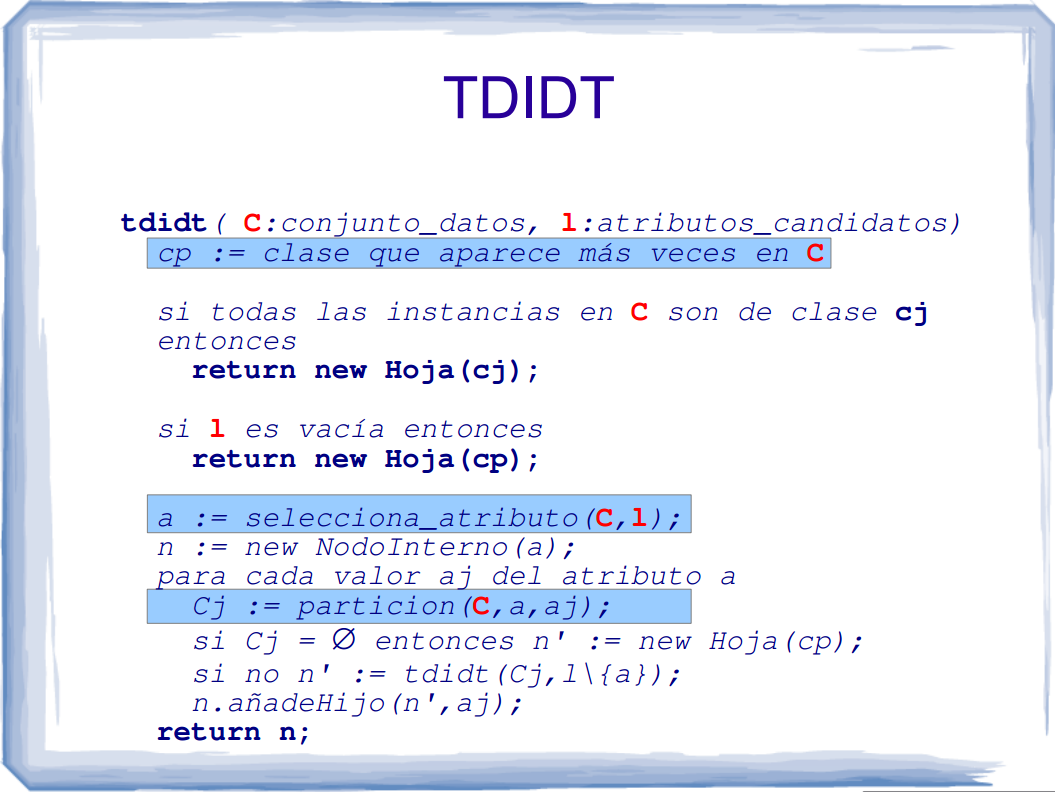
\includegraphics[width=\textwidth]{./images/esquemaTDIDT.png}
\end{frame}

\begin{frame}
  \frametitle{ID3\footnote{Diapositiva sacada del temario de SGDI}}
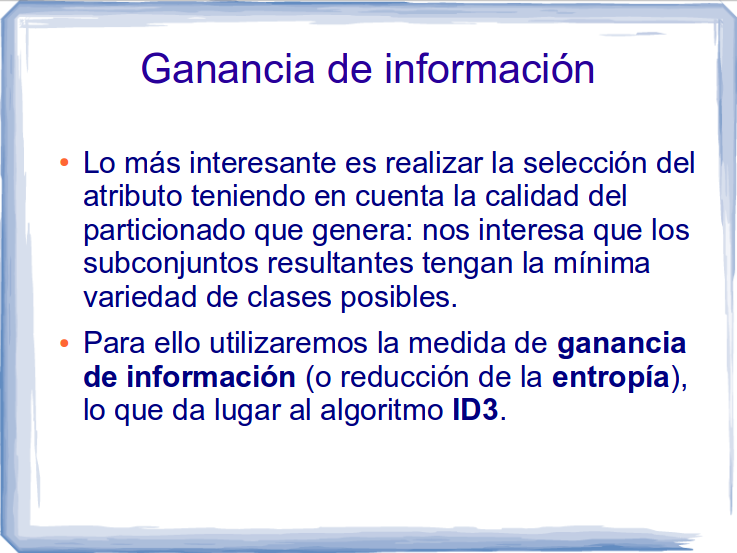
\includegraphics[width=\textwidth]{./images/esquemaID3.png}
\end{frame}

%=================================================
\sectionDark{C4.5}
%=================================================
\begin{frame}
  \frametitle{C4.5}
  El algoritmo ID3 es mejorado por el C4.5. Esta mejora, aparte de la
  optimizaci�n de partes de c�digo, incluye\footnote{Art�culo con las bases del algoritmo \cite{quinlan1986induction}}:
  \begin{itemize}
  \item Permite atributos continuos.
  \item Permite dar un peso diferente a cada atributo.
  \item Permite a una instancia no tener definido un valor en sus
    atributos.
  \item Mejora la selecci�n del atributo clasificador.
  \item Realiza una poda del �rbol despu�s de la creaci�n.
  \end{itemize}
\end{frame}

\begin{frame}[fragile]
  \frametitle{Algoritmo C4.5\footnote{Obtenido del libro \cite{quilan2014c4} y su review \cite{salzberg1994c4}}}
  \begin{tikzpicture}
    \tikzpicdimlarge
    \only<1->{\node[] (def) at (0.5,6) {
        \begin{minipage}{0.9\textwidth}
          \textcolor{purple}{\textbf{Funciones Test:}}
          Para calcular los subconjuntos de instancias al clasificar
          por un atributo se utilizan funciones test de tipo $x >
          40$ � $x < 4$ � $ x = soleado$.
        \end{minipage}
      };}

    \only<2->{\node[] (def) at (0.5,2) {
        \begin{minipage}{0.9\textwidth}
          \textcolor{purple}{\textbf{Selecci�n del atributo:}}
          La selecci�n del atributo por el que dividir consiste en
          escoger el atributo con mayor ganancia de informaci�n
          normalizado y ponderado. \\

          Para ello, se tiene en cuenta la proporci�n de instancias
          que queda en cada rama para el atributo candidato y el peso
          de importancia dado a dicho atributo.\\
          
          La f�rmula queda para el atributo $i$, siendo D el
          conjunto de instancias
          $$ Ganancia_i = Peso_i * \sum_j \frac{|D_j|}{|D|} * Info_j $$
        \end{minipage}
      };}

  \end{tikzpicture}
\end{frame}

\begin{frame}[fragile]
  \frametitle{Ejemplo --  ID3 vs C4.5 (atributos continuos)}
\begin{tikzpicture}
\tikzpicdimlarge
\only<1->{\node[] () at (0,9)
  {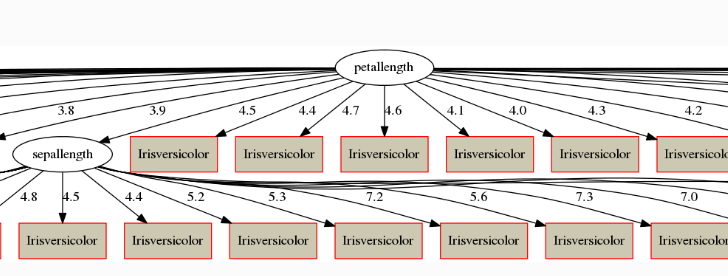
\includegraphics[width=0.65\textwidth]{images/ID3iris.png}};}
\only<2->{\node[] () at (0,5)
  {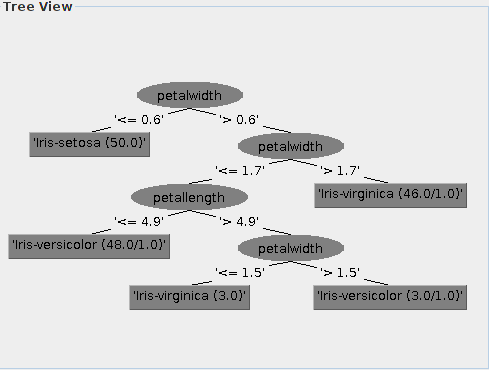
\includegraphics[width=0.65\textwidth]{images/C45tree.png}};}

\end{tikzpicture}
\end{frame}

\begin{frame}
  \frametitle{Mejoras a C4.5}

\end{frame}

%=================================================
\sectionDark{C5.0}
%=================================================

\begin{frame}
  \frametitle{C5.0}
% Mejoras
\end{frame}


%\begin{frame}
%  \frametitle{Ejemplo}
%\end{frame}

%===== EJEMPLO =====
%\begin{frame}[fragile] % Frame ejemplo 2
%  \frametitle{Ejemplo}
%\end{frame}


